\chapter{Model and General Principles}
\label{ch:background}

This chapter will discuss the model and general principles, which serve the foundation to understand the implementation reports of the following chapter. Its important to understand every subsection of this chapter, such as the ethereum blockchain, \ac{PoW}, the \ac{EVM} and all topics needed for atmoic cross-chain swaps. 

% MB NOT HERE - - write about bitcoin and what changes it brought - buterin eth paper

%
% Section: Der erste Abschnitt
%
\section{Ethereum Blockchain}
\label{sec:background:first_section}
The Ethereum blockchain was introduced in Vitalik Buterin’s paper in 2013, which addressed several limitations of the Bitcoin’s scripting language \cite{buterin2013ethereum} based on Buterin's white paper Wood released the yellow paper one year later \cite{wood2014ethereum}. The main contributions are full Turing-completeness and saving all states of computations in between the states \cite{dannen2017introducing}.
Through its own programming language Solidity, it provides an abstract layer enabling anyone to create their own rules for ownership, formats of transactions, and state transition functions \cite{vujivcic2018blockchain}. Development was funded by an online crowdsale that took place between July and August 2014 \cite{tapscott2016blockchain}. The system then went live on 30 July 2015 \footfullcite{"Ethereum Launches" - https://blog.ethereum.org/2015/07/30/ethereum-launches/. Retrieved 30 July 2015} and is called the ethereum public blockchain. Which means its accessible to everyone who wants to send Ether token or execute smart contracts. In general we have to distinguish between private and public blockchains. The public one is described above. Since everybody can go to github and fork e.g the geth client its possible to start an own private blockchain. In an enterprise software context, where corporate stakeholders are given certain rights and privileges to read and write to the company chain, the deployment is known as a permissioned blockchain. Nevertheless for both the private (permissioned) and the public blockchain its possible to do the following \cite{dannen2017introducing}:

\begin{itemize}
	\item Send and receive Ether
	\item Write smart contracts
	\item Create provably fair applications
	\item Launch your own token based on Ether
\end{itemize}

% ADD LINEBREAK TO FOOTNOTE AND ADD THIS AT THE BEGINNING   Foundation, Ethereum 

\clearpage

\subsection{Proof-of-Work Consensus Algorithm}
\label{subsec:background:first_section:second_subsection}

%MB check wood paper for more historical PoW data!!

The \ac{PoW} system of bitcoin and ethereum is similar to Adam Back's Hashcash \cite{back2002hashcash}, but instead of a newspaper or Usenet post the \ac{PoW} involves scanning for a value, which is hashed with the \ac{SHA-256} to begin with a number of zero bits. The average work required is exponential. Which means the more leading zeros, the more work. In the end the work can be later verified by executing a single hash. The \ac{PoW} is implemented by incrementing a nonce in the block until a value is found that gives the block's hash the required zero bits. The majority decision is represented by the longest chain, which has the greatest \ac{PoW} effort invested in it. Because later blocks are chained after the premature block, the work to change the block would include redoing all the blocks after it. To modify a past block, an attacker would need to redo all the past work until the specific block he wants to change \cite{nakamoto2008peer}. 

\begin{figure}[h]
	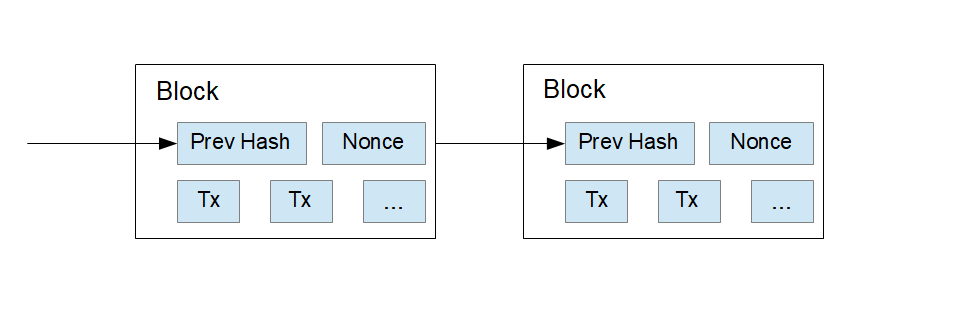
\includegraphics[height=4cm]{blocks}
	\caption{Blocks}
	\label{fig:blocks}
\end{figure}

Beginning with the genesis block, each single block is chained to the previous block by including the the previous hashes (figure \ref{fig:blocks}). The \ac{SHA-256} takes a 256 bit length of input
messages and hash them to fixed-length outputs \cite{van2014encyclopedia}. So the \ac{SHA-256} function starts by padding the message according to the so-called Merkle-Damg{\aa}rd strengthening technique. Further the message is processed block by block with the the underlying compression function, which initializes an appropriate number of chaining variables to a fixed value to hash the genesis block and also the current hash value for the following blocks \cite{coron2005merkle}. In the year 2003 the \ac{SHA} was published by the \ac{ISO} making \ac{SHA} a standard for most countries in the world \cite{isoSHA-256}. Five years later Satoshi Nakamoto proposed the first concept of a \ac{PoW} based blockchain to allow for public agreement on the order of transactions. The public ethereum blockchain uses \ac{PoW} to this day. There are several other consensus algorithms today suitable for a blockchain and some are considered to be an improvement to \ac{PoW}, which will be discussed later in this work.

\clearpage

\subsection{Ethereum Virtual Machine}
\label{subsec:background:first_section:ethereum}
This chapter will cover basics of the \ac{EVM} and discuss the transaction execution to reach a general understanding what the \ac{EVM} is and how it works. The \ac{EVM} is a simple stack-based architecture. The word size of the machine is 256-bit and the stack has a maximum size of 1024 elements, meaning that the \ac{EVM} can store a total of 1024 stack items with each 256-bit. The machine does not follow the standard von Neumann architecture. Rather than storing program code in generally-accessible memory or storage, it is stored separately in a virtual ROM. The \ac{EVM} is different from the von Neumann architecure, because it can have exceptional execution thus as the out-of-gas exception. \cite{wood2014ethereum} The ethereum network can be seen as one single computational device, where the point of turning the machine on is the creation of the genesis block. All blocks of a blockchain hold information about state changes of the \ac{EVM}, the ethereum public blockchain holds all state transitions of the \ac{EVM} since it was initially turned on. Since every state transition of the \ac{EVM} is modelled as a transaction, a blockchain holds the whole history of states of the specific machine \cite{dannen2017introducing}. Before it will be put into a block each transaction is verified and validated before the next canonical block can be placed on the last one. Through the transaction validation, nodes on the network do not need to individually evaluate the trustworthiness of every single block in the network to compute the present balances of the accounts on the network. The client simply has to verify the hash of the parent block and see if the new block contains the correct hash its parent’s transactions and state \cite{dannen2017introducing}. The current valid block in an ethereum network is known as world state (state), which is a mapping between addresses (160-bit identifiers) and account states. Thus being the current executional state of the virtual state machin, knwon as the \ac{EVM}. It is considered as a quasi-Touringcomplete virtual machine. Since the amount of total execution is intrinsically bound to the parameter gas, the quasi  qualification is added \cite{wood2014ethereum}. The execution model is defined by the ethereum state transition function and specifies how system state is altered through bytecode executions. \newline \newline
The ethereum state transition function, APPLY(S, TX) -> S' is defined by Buterin \cite{buterin2013ethereum}  as follows:

\begin{enumerate}
	\item Check for transaction and signature validity and check if the nonce of the sender account matches the receivers account's nonce. If not, return an error.
	\item Calculate the transaction fee and determine the sending address from the signature. Increment the sender's nonce and substract the fee from the sender's account. Return an error, if the balance of the sender's account is lower than the fee.
	\item Initialize GAS including a certain quantity of gas per byte to pay for the bytes in the transaction.
	\item If the receiver's account doesnt exist, create it and then send the transaction value from sender's account to the receiver. If the receiver's account is a contract, run code execution until completed or gas is depleted.
	\item In case the value transfer or code execution failed because theres not enough gas, revert all state changes except the payment of the fees and add the fees to the miner's account.
	\item If code execution has completed refund the fees for all remaining gas to the sender and also send the fees paid for gas consumed to the miner.
\end{enumerate}


\begin{figure}[h]
	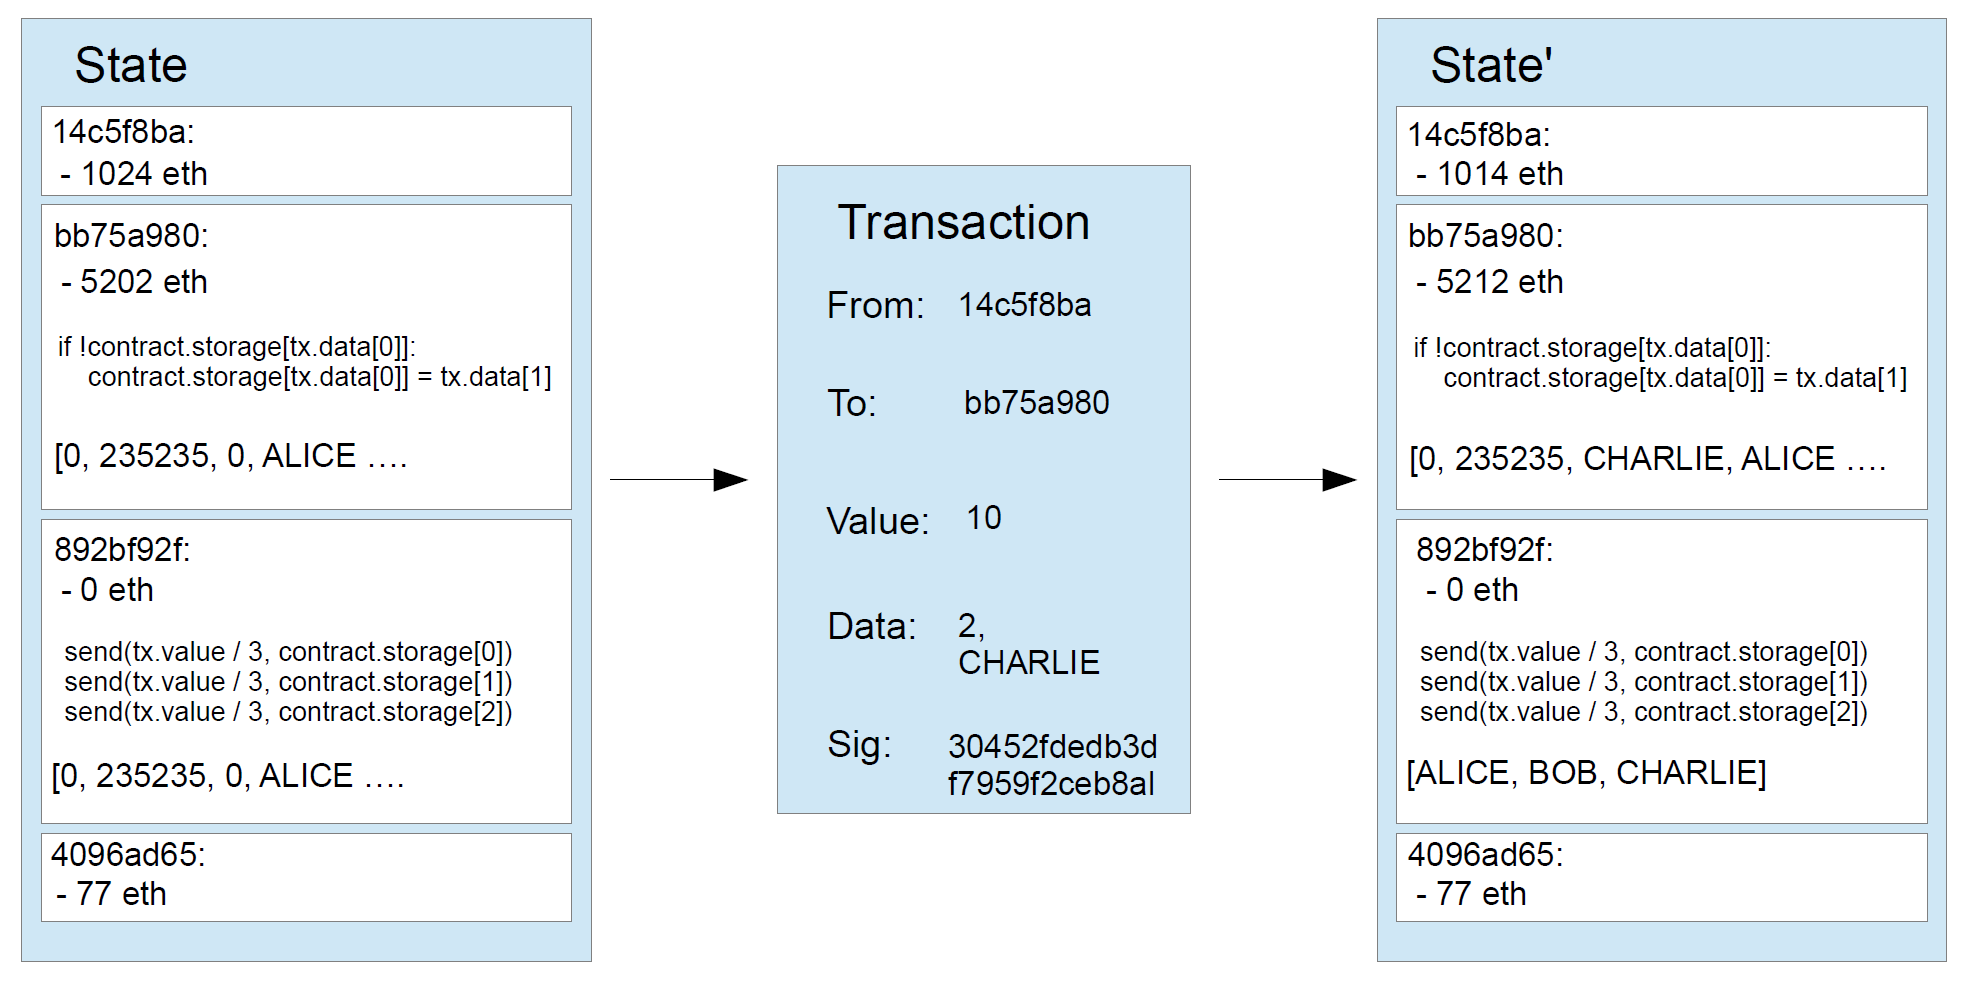
\includegraphics[width=14cm]{ethereum_state_transition_function}	%16cm
	\caption{Ethereum State Transition Function}
	\label{fig:ethereum_state_transition_function}
\end{figure}
% BRING REAL EXAMPLE WITH CALCULATIONS OF GAS?

The Figure above shows all calculations applying the function APPLY(S, TX) -> S' to an example state (figure \ref{fig:ethereum_state_transition_function}). Due to the distributed nature of the \ac{EVM} and the fact its built of many nodes around the world. Meaning to ensure distributed security, it must be purpose-built to solve the diffmatching problem that can occur, when there are many near-simultaneous changes to the same database from many actors in the system all around the world \footfullcite{Google Code "Diff-Match Patch" - https://code.google.com/p/google-diff-match-patch/ 2016}. Solving this problem in a verifiable and trustworthy way is basically what the \ac{EVM} does. It's resilience and security does increase with the amount of machines in the network and is implemented and backed by the gas fee system. The opportunity to earn gas as a miner is one reason for many nodes to participate in the network and at the same time raises security \cite{dannen2017introducing}.

% MB add that there are opcodes and stuff, like any other machine has, but not covered here(would go too deep)
%- explain how code execution works on a distributed system

%ueberleitung von execution model erledigt zur smart contract 
 
\clearpage


\subsection{Smart Contracts}
\label{subsec:background:first_section:first_subsection}
Around the 1990s it became clear that algorithmic enforcement of agreements could become common in the way humans cooperate. Early work towards smart contracts was done by Szabo \cite{szabo1997formalizing} and Mark Miller \cite{miller1997future}. Even though no specific system was proposed by them, they proposed that the future of law would be driven by such systems. Ethereum can be seen as such a system, it delivers a general implementation to execute financial contracts by a machine. The term smart contract was first introduced by Buterin \cite{buterin2013ethereum}, in scientific context they are simply called contracts by Wood \cite{wood2014ethereum}. In this context, contract refers to a specific kind of contract: a financial contract, also known as derivative or option. These contracts are agreements between two parties to buy or sell a specific asset at some point in the future or when certain conditions are met, like a specified price. In ethereum context a contract does basically the same thing as a financial contract. The contract is written as code and is an agreement between accounts, to send a payment to a specified address, when certain conditions are met. The reason these contracts are called smart contracts, is because they are executed by a machine, also known as the \ac{EVM}. When certain conditions are met, the assets (ether or token) will be moved automatically by the machine. Assuming the system is still running, these smart contracts can also take effect hundreds of years after being deployed. As long as the \ac{EVM} is running, deployed contract maintain their validity. Its basically impossible for a party to back out of these contracts, because the smart contracts are empowered to move or hold assets and move them to specific accounts when the implemented conditions are met \cite{dannen2017introducing}. While smart contract are often written in the high level programming language solidity, the code the \ac{EVM} understands and executes is written in a low-level, stack based bytecode language, referred to as \ac{EVM Code}. In general the bytecode consists of a series of bytes, where each byte represents an operation to be executed by the \ac{EVM} and code execution is an infinite loop executing code and storing data to the following operations until an error or STOP or RETURN is reached \cite{buterin2013ethereum}:

\begin{itemize}
	\item Stack (last-in-first-out container to which 32-byte values are pushed or popped)
	\item Memory (infinitely expandable byte array)
	\item Storage (of a contract, changes here don't reset after computation ends they are persistent)
\end{itemize}

%MB add further information about code execution!!

\clearpage


\section{Digraphs}
\label{sec:background:second_section}
A \ac{digraph} D (figure \ref{fig:a_digraph_d}) in the example consists of a finite nonempty set of objects called vertices. So the vertex set of the example \ref{fig:a_digraph_d} is V(D) = \{u, v, w, x, y, z\}. It also has a finite set of A(D) of ordered pairs of distinct vertices called arcs (or directed edges according to \cite{chartrand2010graphs}), in this example \ref{fig:a_digraph_d} A(D) = \{(u, v), (u, w), (w, u), (z, u), (x, z), (y, z)\}. So the \ac{digraph} D consists of V(D) the vertex set and A(D) the arc set of D, which can also be expressed as D = (A, V). \newline



\begin{figure}[h]
	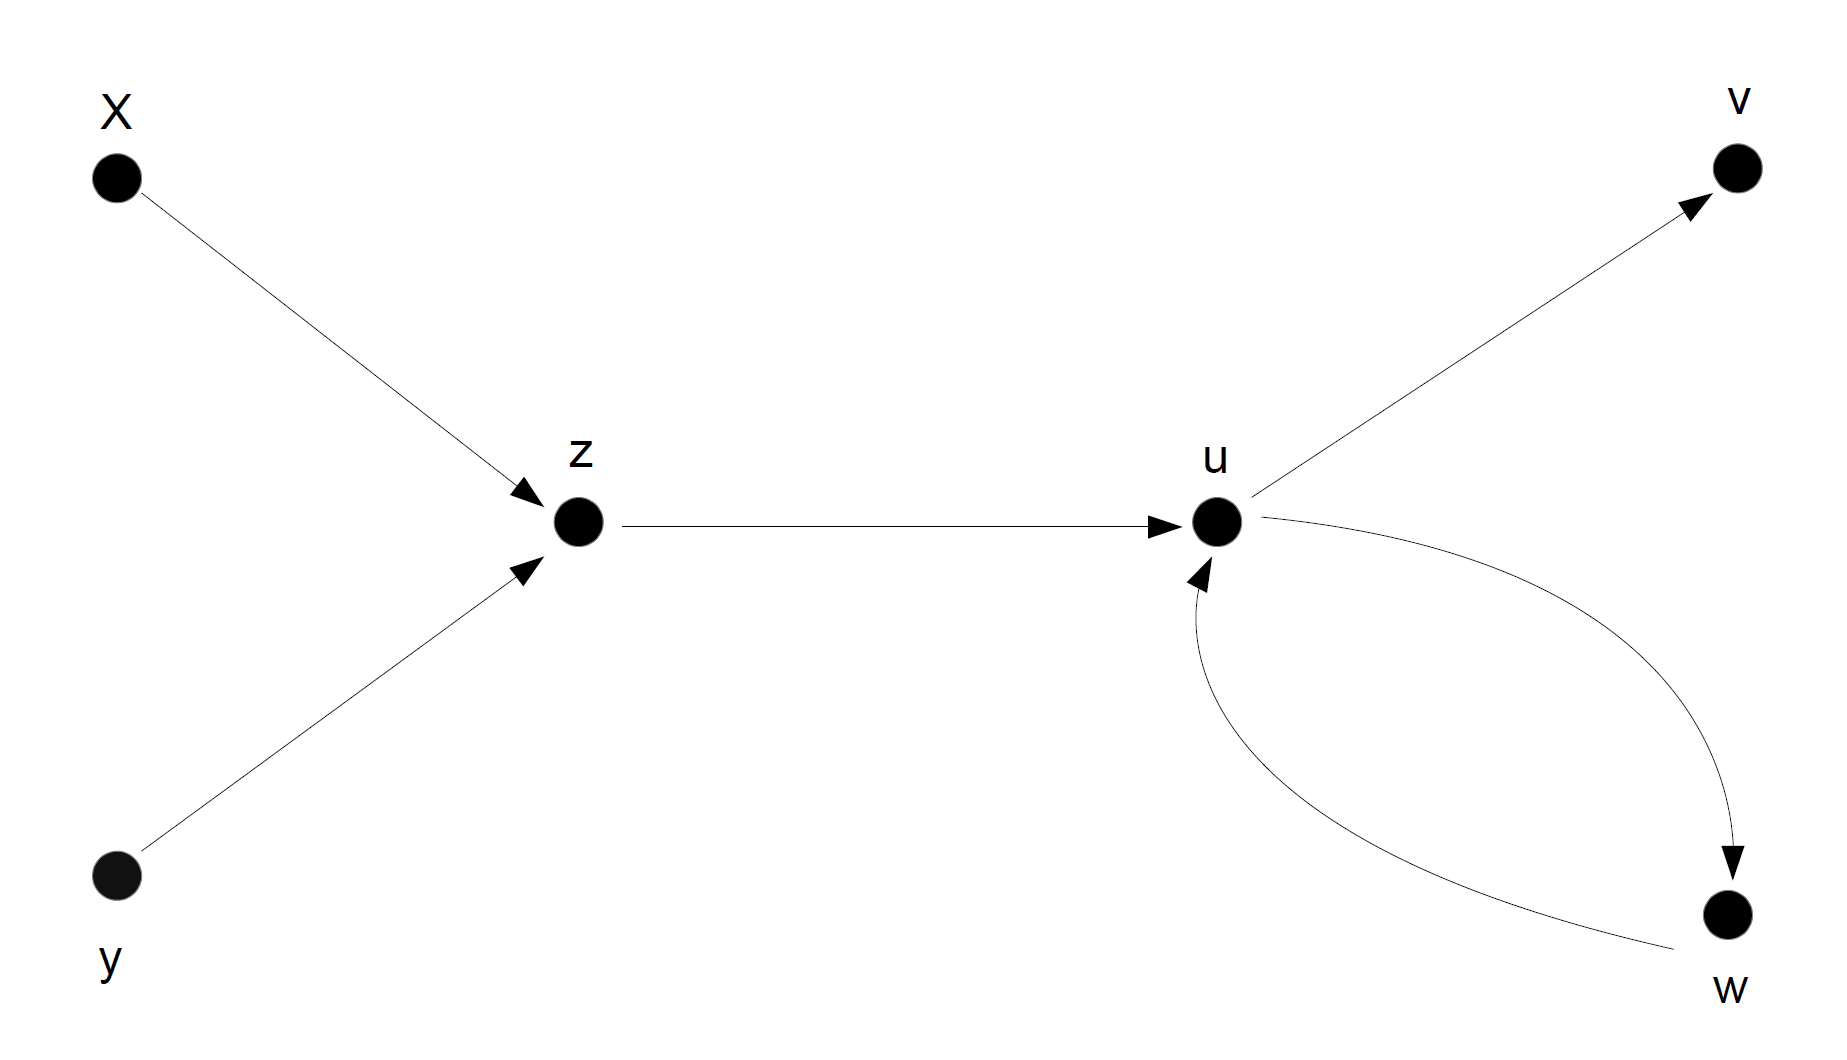
\includegraphics[height=7cm]{adigraphd}	%16cm
	\caption{A Digraph D}
	\label{fig:a_digraph_d}
\end{figure}


The order (size) is sometimes denoted as |D|, so th e size of the \ac{digraph} D in the example \ref{fig:a_digraph_d} is |D| = 6. For an arc (u, v) the first vertex u is its tail and the second vertex v is its head, we can also day that the arc (u, v) leaves u and enters v. Another expression is, assuming (u, v) is an arc, one can say that u dominates v (or v is dominated by u) and can be denoted by u -> v \cite{bang2007theory}. The example in this chapter and its figure \ref{fig:a_digraph_d} is important to understand and know the basic terminology, since the processes of atomic cross-chain swaps itself is are a combination of two digraphs.

%TODO: explain aclyclic digraph and strongly connected and feedback vertex

%TODO: strongly connected: A digraph D
%is strongly connected (or, just, strong) if, for every pair x; y of distinct
%vertices in D, there exists an (x; y)-walk and a (y; x)-walk. In other words,
%D is strong if every vertex of D is reachable from every other vertex of D.

%TODO: acyclic
%A digraph D is acyclic if it has no cycle(doesnt loop). -> ref to \cite{bang2007theory}

%TODO: feedback vertex
%In a digraph D, a set S of vertices (arcs) is a feedback ver-
%tex set (an feedback arc set) if D ¡ S is acyclic.

% The head and tail of an arc are its end-vertices; we say that the end-vertices are adjacent, i.e. u is adjacent to1 v and v is adjacent to u.
% MB needs more explanation and terminology.
\clearpage

\section{Atomic Cross-Chain Swaps}
\label{sec:background:fifth_section}
%implementation later on will follow the concept of herlihy.
An atomic cross-chain swap is like the name indicates an atomic transaction to swap assets, which is also across multiple blockchains. Altough ethereum can be seen as one system, its still a distributed ledger, so the atomic cross-chain swap is a distributed coordination task (special case of distributed atomic transaction) \cite{weikum2001transactional}. Since the swap is atomic it either finishes the protocol or initiate refunds in case any party doesn't follow through the whole protocol. The concept of atomic cross-chain swaps is well known to the blockchain community and will be discussed later on in \autoref{ch:chapter03} (Related Work). All following concepts and models discussed are based on Herlihy's work \cite{herlihy2018atomic}. A cross-chain swap is modeled as a directed graph D, the vertexes of the digraph represent the parties and its arcs are proposed asset transfers. For any pair(D,L), where D = (V,A) is a strongly-connected directed graph and L (subset) V a feedback vertex set for D. The three-way swap in specific has to be an acyclic and utilitizes a slightly modified form of a digraph introducing followers and leaders and using a form of hashed timelock contracts, read more in \autoref{subsec:background:second_section:hashlock_timelock}. The concept of atomic cross-chain swaps removes the intermediate party, which is usually an exchange marketplace for cryptocurrencies to trade assets or tokens. This chapter starts with an example of a three-way swap (\autoref{subsec:background:second_section:example}), discussing the model of hashlocks and hashkeys (\autoref{subsec:background:second_section:hashlock_timelock}) and at last propose a general protocol (\autoref{subsec:background:second_section:protocol}) for three-way swaps.

%TODO insert subset symbol to (subset)

\subsection{Example}
\label{subsec:background:second_section:example}
%next subchaptes will discuss the underlying model, which allows the three parties in the following example to exchange their assets or funds across three blockchains. Since its an atomic transaction no party will end up bad, if one party doesnt apply to the protocol or something goes wrong. The swap will either be completed or all funds will be returned after a certain amount of time.

Lets assume Carol lifes in a state where car titles are managed on a blockchain and wants to sell her car for bitcoins. Alice is interested in Carol's car, but wants to pay in another cryptocurreny(following called alt-coin). Lucky for both that Bob is willing to trade his alt-coins for bitcoins. Since none of the parties trust each other, they can arrange a three way swap to assure their transaction is atomic across the different blockchains. To complete the transaction Alice has to send her alt-coins to Bob, so he can transfer his bitcoin to Carol who will finally give the car to Alice. If all parties stick to the deal then everything will be fine, to assure that no one looses their funds due to a malicious actor who behaves irrationally this chapter and the following will discuss the protocol of atomic cross-chain swaps by the example of Alice, Bob and Carol's transaction. Today many blockchains come with smart contracts to execute a transfer of funds if certain conditions are met.
Let H(. / replace with other dot!) be a cryptographic hash function. Alice could transfer her alt-coins to a smart contract which acts as escrow on the alt-coin blockchain, the contract also holds the information of hashlock h and timelock t. The hashlock h is determined by a contract value s, called a secret and let h = H(s). If Alice sends the secret to Bob it allows him to claim the funds sitting in the smart contract's escrow using hashlock h. Timelock t means that Bob also needs to produce a secret before the time t elapsed, if he doesnt manage to prduce the secret in time, then the funds on the alt-coin blockchain are transfered back to Alice by the smart contract. Let (triangle) be enough time for the parties to publish their smart contracts or detect changes. Since Alice, Bob and Carol need to execute a three-way swap illustrated in figures \ref{fig:deploying_contracts} and \ref{fig:triggering_arcs} they need to apply to the following simple protocol: \newline

%TODO insert Delta Δ

\begin{itemize}
	\item Alice publishes a smart contract on the alt-coin blockchain including a secret s, h = H(s) she created. The contract also holds the information of hashlock h and timelock 6(triangle) in the future, to send her alt-coins to Bob.
	\item As soon as Alice's contract is confirmed on the alt-coin blockchain and detected by Bob, he deploys a smart contract on the bitcoin blockchain to transfer his funds to Alice. Bob adds the same hashlock h value to the contract like Alice and a timelock 5(triangle) in the future.
	\item When Carol detects Bob's confirmed smart contract on the bitcoin blockchain, she publishes a smart contract on the car title blockchain in order to transfer the title of her car to Alice. Again with same hashlock h, but timelock 4(triangle) in the future
	\item After Alice confirms Bob's mined contract on the title blockchain, she sends s to Carol's contract. Alice aquires the title and reveals s to Carol.
	\item Carol then sends s to Bob's contract, she aquires the bitcoin and reveals s to Bob.
	\item Bob completes the swap by sending s to Alice's contract and claiming the alt-coins.
\end{itemize}

\begin{figure}[h]
	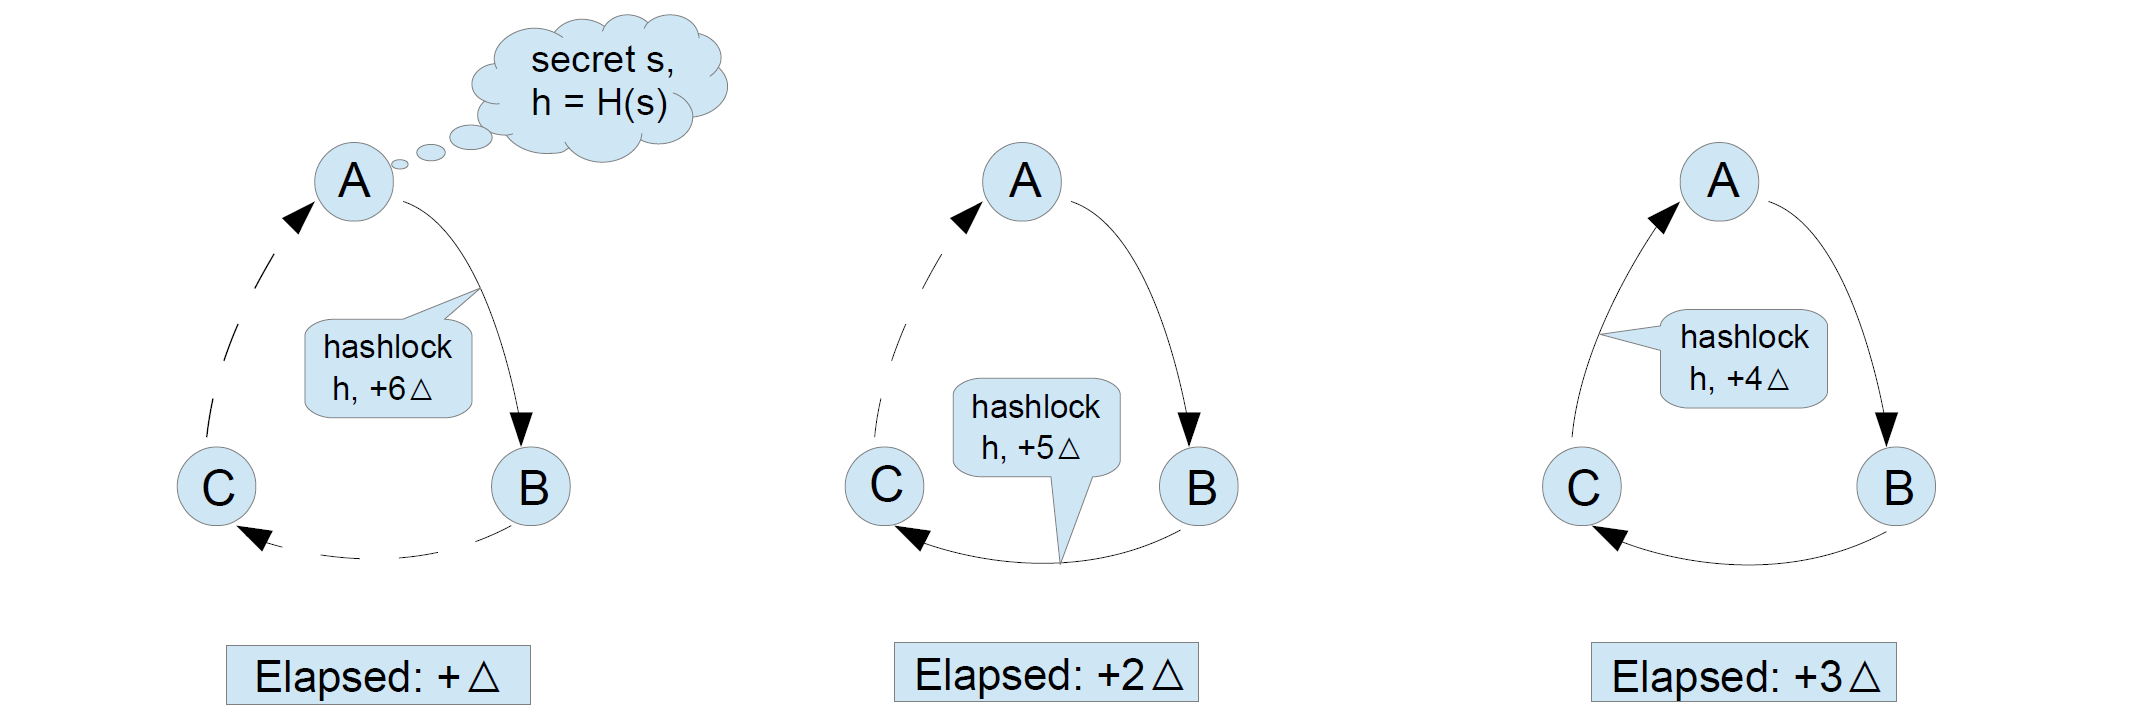
\includegraphics[width=16cm]{deploying_contracts}	%16cm
	\caption{Atomic cross-chain swap: deploying contracts}
	\label{fig:deploying_contracts}
\end{figure}

\begin{figure}[h]
	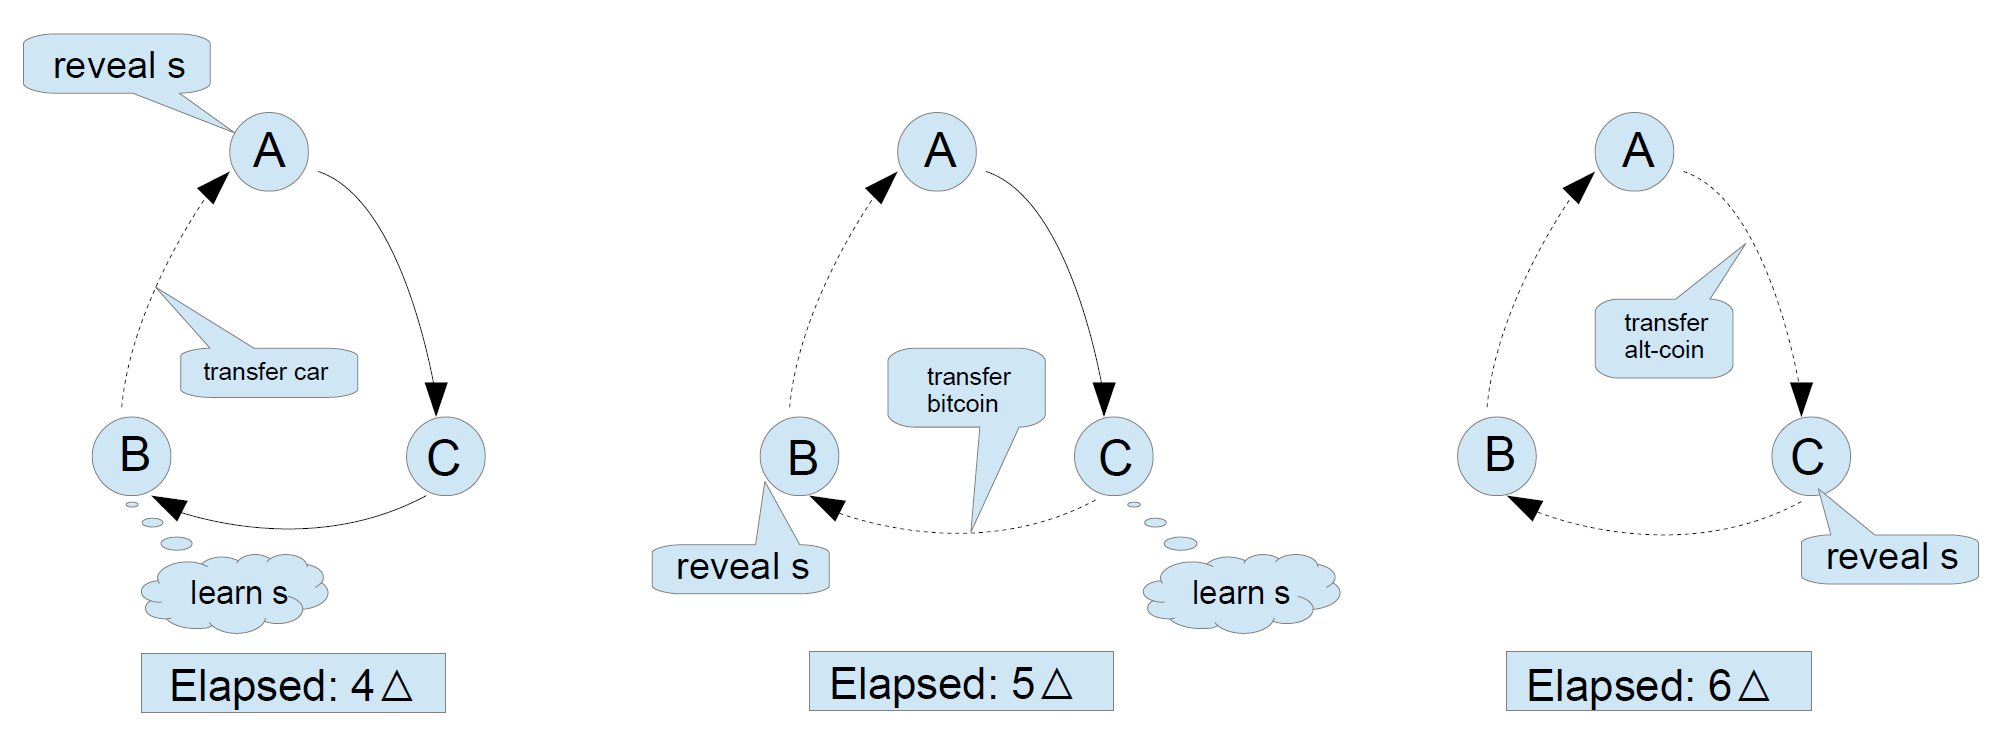
\includegraphics[width=16cm]{triggering_arcs}	%16cm
	\caption{Atomic cross-chain swap: triggering arcs}
	\label{fig:triggering_arcs}
\end{figure}


So what could possibly go wrong in this three-way swap? If any party fails to publish their contract during deployment phase, then all contracts will timeout and trigger refunds of the assets. If any party fails while triggering arcs, then only that party will end off worse. For example, if Carol halts execution of the swap without triggering her contract, then Alice gets the car and Bob gets a refund. So in that case Carol would only harm herself. Also the order of contract's deployment matters. Because if Carol posts her contract with Alice, before Bob posts his contract with Carol, then Alice could claim the car title without paying Carol. The timelock values are also important. For example, if Carol's contract with Bob and Bob's contract with Alice would expire at the same time, then Carol would reveal s to collect Bob's bitcoin at the very last moment, leaving Bob no time to claim his alt-coins from Alice. If parties behave irrationally, then Alice might end up not getting her car. This would be the case if Alice (irrationally) reveals s before phase completion, then Bob can take Alice's alt-coin and Carol might be able to take Bob's bitcoin.
%TODO: lookup refs in swaps paper and add one or two sentences why this is an active research field.


\subsection{Hashlocks and Hashkeys}
\label{subsec:background:second_section:hashlock_timelock}

%add as footnote:
%[5] bitcoinwiki. Hashed timelock contracts. hŠps://en.bitcoin.it/wiki/HashedTimelock Contracts. As of 8 January 2018.

\cite{li2019research}

\begin{figure}[h]
	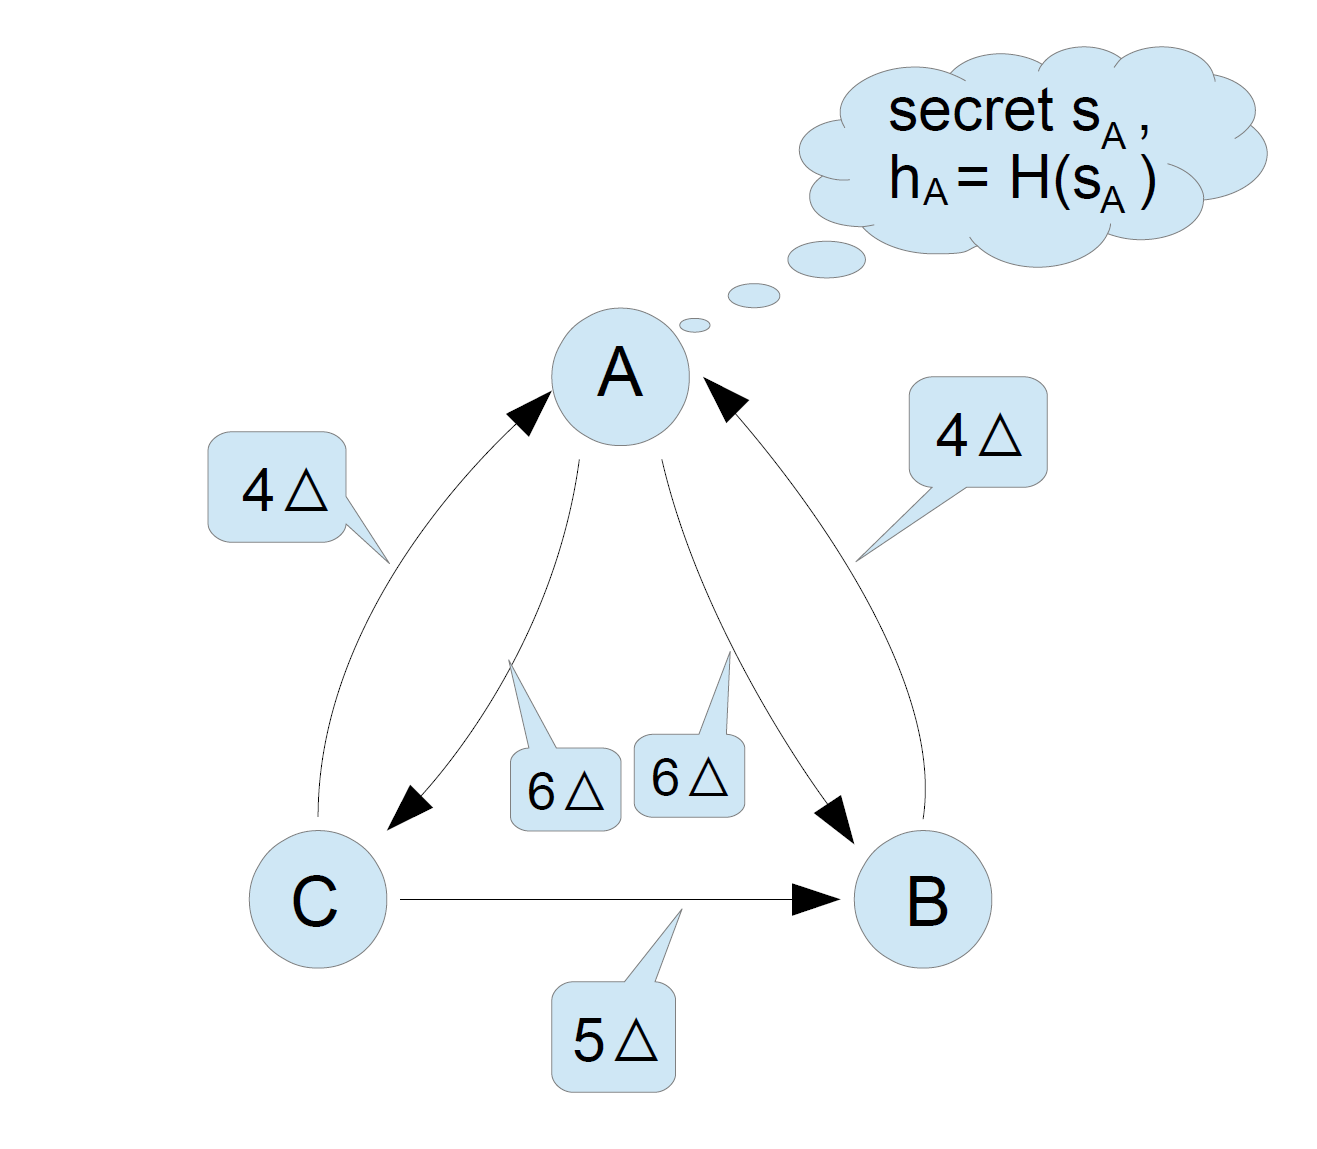
\includegraphics[height=9cm]{acyclic_timeouts}	%16cm
	\caption{Acyclic subdigraph with assigned timeouts (A is the leader, B and C followers)}
	\label{fig:acyclic_timeouts}
\end{figure}



\subsection{The Protocol}
\label{subsec:background:second_section:protocol}


\begin{figure}[h]
	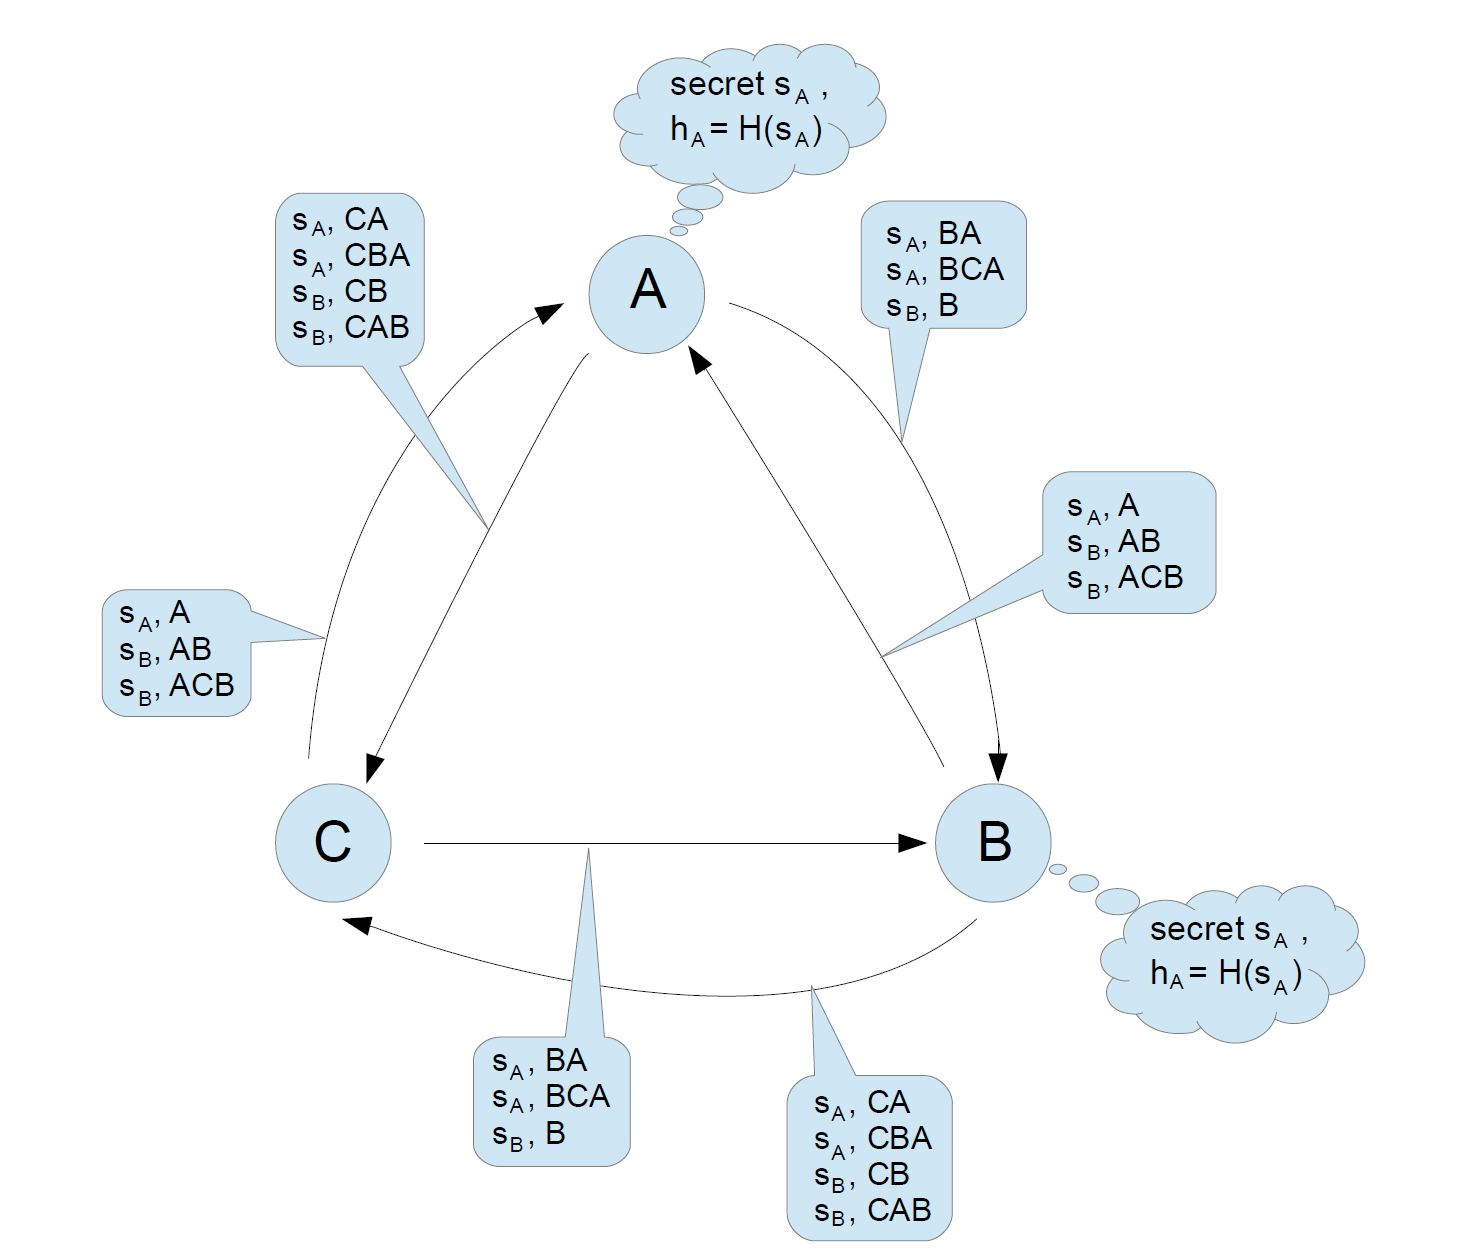
\includegraphics[height=8cm]{hashkey_paths}	%16cm
	\caption{Hashkey paths for arcs of two-leader digraph}
	\label{fig:hashkey_paths}
\end{figure}
